\chapter{Background}
\label{ch:Foundation}
\section{Background on EEG}
\label{sec:Background:Background on EEG}
Developing a direct interface for communication and control between human brains and computers has been a subject of contemplation within the scientific community for an extended period. Numerous research and development initiatives have been employed to actualize this concept, resulting in its emergence as a highly burgeoning field of scientific investigation in recent times \cite{clinical_trails}. This vast area of research has also led to the development of something now known as Brain-Computer Interface (BCI). BCI technologies have been widely utilized in the healthcare industry. These technologies have been applied in various tasks, including fatigue detection, assessment of sleep quality, and clinical applications such as detecting and predicting abnormal brain diseases. Examples of these diseases include seizure disorders, Parkinson's disease, Alzheimer's disease, and schizophrenia. \cite{BCI_applications}.
\smallskip

BCI can be classified into three groups: invasive, partially invasive, and non-invasive. The first two classifications of BCIs necessitate the surgical placement of sensors(electrodes) within the brain cortex to capture the minute currents produced due to cerebral responses. Although invasive methods of BCI provide superior signal quality, the surgical dangers and requirement for long-term installation of invasive devices offset any potential benefit of improved signal quality \cite{velasco2019bci}. 
%On the other hand, non-invasive technology utilizes external neuroimaging devices to record brain activities, consisting of functional near-infrared spectroscopy (fNIRS), functional magnetic resonance imaging (fMRI), and electroencephalography (EEG). Non-invasive EEG-based devices have been the most widely utilized modality for practical BCIs and clinical applications due to the relative improvements in signal quality, dependability, and mobility compared with alternative imaging techniques
In contrast, non-invasive technology involves external neuroimaging devices to capture brain processes. This includes functional near-infrared spectroscopy (fNIRS), functional magnetic resonance imaging (fMRI), and electroencephalography (EEG). Utilizing non-invasive devices based on EEG has been prevalent in practical BCIs and clinical applications. This is mainly owing to the notable enhancements in signal quality, reliability, and portability compared to other imaging techniques \cite{BCI_applications}. The proliferation of affordable and highly portable EEG equipment, exemplified by various consumer devices such as Neurosky\footnote{\url{https://neurosky.com/}}, has expanded the application of BCIs beyond the confines of the healthcare industry and into domains such as gaming. Research on brain biometrics has recently garnered a lot of attention in this area, which has been further encouraged by the limitations of using passwords to prove online identity \cite{arias2021inexpensive}.  


\section{EEG Instruments and Data Acquisition}
\label{sec:Background:EEG Instruments and Data Acquisition}

\begin{figure}%
    \centering
    \subfloat[\centering Medical grade EEG headset from g.tec ]{{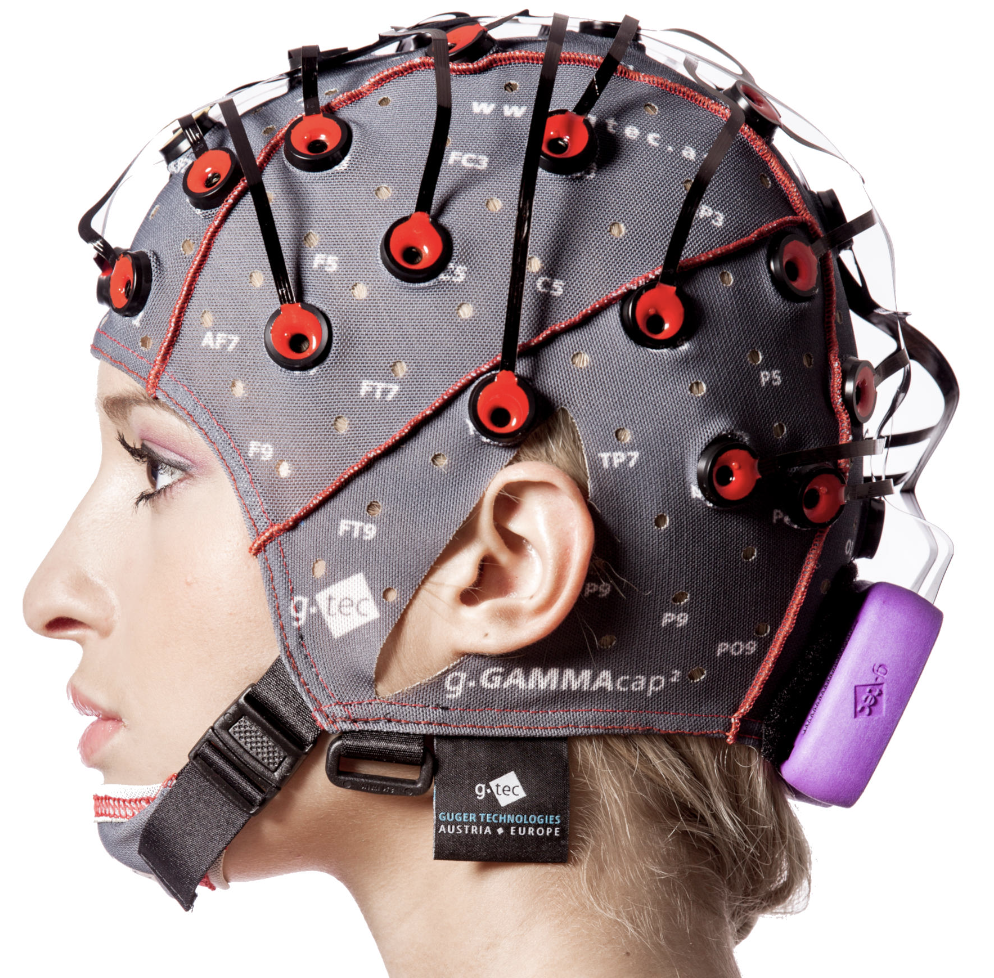
\includegraphics[width=7.55cm]{figures/Headset/g.tec headset.png}}}%
    \qquad
    \subfloat[\centering EPOC/EPOC+ wearable headset]{{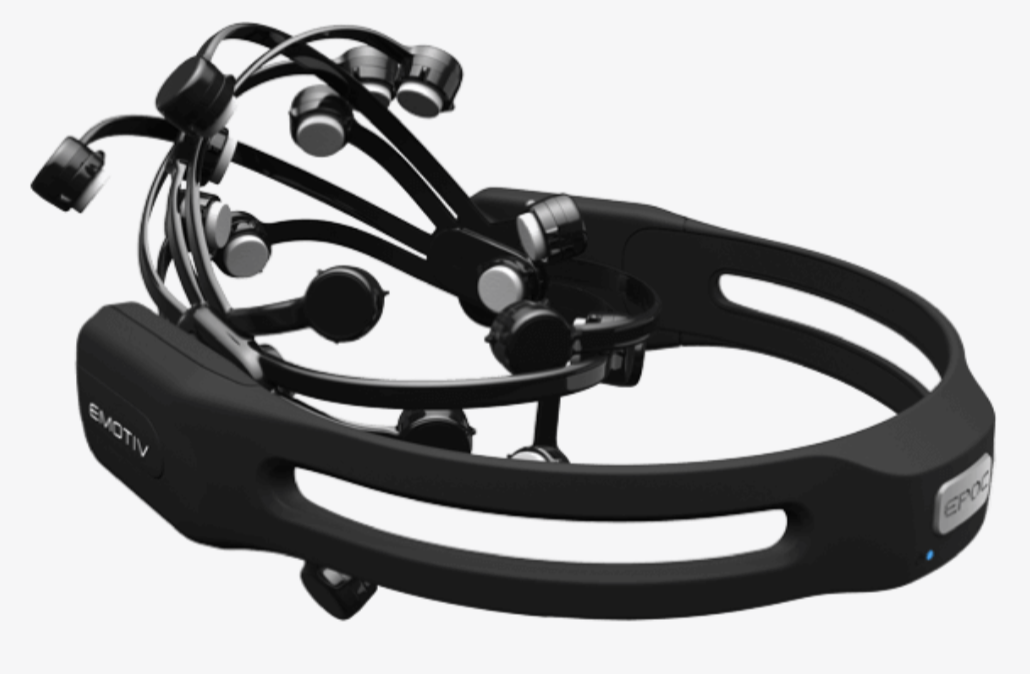
\includegraphics[width=7.55cm]{figures/Headset/Emotiv Comsumer Device.png} }}%
    \caption{In Figure (a), we can observe the g.GAMMAcap, which is among the frequently utilized medical-grade EEG headsets. Moving on to Figure (b), we see the EMOTIV EPOC+ device equipped with 14 EEG electrodes. }
    \label{fig: Headsets}%
\end{figure}
To acquire the EEG) signals, an EEG apparatus necessitates the inclusion of sensors capable of establishing conductive contact with the scalp. This amplifier facilitates real-time filtering and common mode rejection, an analog-to-digital converter (A/D converter), and a personal computer (PC) to store the digitized data \cite{survey_brain_biometrics}. The EEG headset, which records the brain activity, includes sensors arranged according to the 10-20 or 10-10 system, which are international standards for consistent placement of electrodes, ensuring comparability across subjects and studies. The naming of the electrodes within these systems follows a specific convention that represents the brain region underneath (e.g., 'F' for frontal, 'C' for central) and an odd or even number indicating the hemisphere (odd for left, even for right) \cite{abhang2016introduction}. Frequently utilized EEG devices include the ActiveTwoSystem designed by Biosemi (Amsterdam, Netherlands)\footnote{\url{http://www.biosemi.com/}} and the g.GAMMAcap developed by G.Tech Medical Engineering GmbH\footnote{\url{https://www.gtec.at/}}. An example EEG headset from G.Tech is illustrated in Figure \ref{fig: Headsets} (a). These medical-grade EEG systems can support up to 256 channels, allowing for comprehensive data collection. This feature offers a benefit as it facilitates a greater extent of spatial coverage on the scalp, resulting in a more comprehensive dataset \cite{survey_brain_biometrics}.
\smallskip

Although medical-grade EEG devices are known for their ability to gather data of high quality, the considerable expense associated with these devices and the complexities needed in establishing the EEG connection pose notable obstacles. In response to these constraints, there has been a proliferation of cost-effective and user-accessible EEG devices in recent times, presenting viable substitutes. Instances of such devices include the ENOBIO developed by Neuroelectrics (Barcelona, Spain)\footnote{\url{https://www.neuroelectrics.com/}}, the EPOC/EPOC+ wearable neuroheadset designed by Emotiv Systems, Inc. (San Francisco, USA)\footnote{\url{https://www.emotiv.com/epoc/}}, along with the Muse headband crafted by InteraXon (Ontario, Canada)\footnote{\url{https://choosemuse.com/}}. An EPOC/EPOC+ wearable EEG headset equipped with 14 sensors is depicted in Figure \ref{fig: Headsets} (b). Consumer devices are cheaper than medical-grade EEG headsets and more friendly but have a poor signal-to-noise ratio \cite{survey_brain_biometrics}. 

%Examples of these are the ENOBIO developed by Neuroelectrics (Barcelona, Spain)\footnote{\url{https://www.neuroelectrics.com/}}, the EPOC/EPOC+ wearable neuroheadset developed by Emotiv Systems, Inc. (San Francisco, USA)\footnote{\url{https://www.emotiv.com/epoc/}}, and the MindWave wearable headset developed by NeuroSky, Inc. (San Jose, USA) and Muse headband developed by InteraXon (Ontario, Canada). 


%BCI can be classified into three groups: invasive, partially invasive, and non-invasive. The former two categories of BCI require surgically inserting electrodes into the brain cortex to record the small currents generated due to brain responses. BCI can be classified into three groups: invasive, partially invasive, and non-invasive. The former two categories of BCI require surgically inserting electrodes into the brain cortex to record the small currents generated due to brain responses. 
% \begin{itemize}
% \item For EEG acquisition, an EEG device must incorporate sensors that can establish a conductive connection with the scalp. This device also requires a bio amplifier for real-time filtering and common mode rejection, an A/D converter for digital translation, and a computer system for storing the converted data.
% \item The headset includes sensors arranged according to the 10-20 or 10-10 system, which are international standards for consistent placement of electrodes, ensuring comparability across subjects and studies. These systems provide comprehensive coverage, allowing for detailed EEG data collection.

% \item The naming of the electrodes within these systems follows a specific convention that represents the brain region underneath (e.g., 'F' for frontal, 'C' for central) and an odd or even number indicating the hemisphere (odd for left, even for right).

% \item The EEG headsets can be medical grade, such as ActiveTwoSystem by Biosemi (Amsterdam, Netherlands) or g.USBamp (G.Tech Medical Engineering GmbH. These medical-grade EEG devices can accommodate as many as 256 channels. One of the main disadvantages of using these devices is the longer preparation time. They are also costly.

% \item Recent advances in neurotechnology have led to the development of cheap and consumer-friendliness. Examples of these are the ENOBIO developed by Neuroelectrics (Barcelona, Spain)2, the EPOC/EPOC+ wearable neuroheadset developed by Emotiv Systems, Inc. (San Francisco, USA)3, and the MindWave wearable headset developed by NeuroSky, Inc. (San Jose, USA) and Muse headband developed by InteraXon (Ontario, Canada). Consumer devices are cheaper than medical-grade EEG headsets and more friendly but have a poor signal-to-noise ratio. 
% \end{itemize}

\section{Data Acquisition Procedures}
\label{sec:Background:Data Acquisition Procedures}
%EEG recording can be done 
% \begin{itemize}
The firing of neurons in the brain is significantly influenced by the mental state of individuals, exhibiting a solid susceptibility to both external environmental stimuli and internal self-regulation. Hence, it is imperative to devise a specialized collecting paradigm to gather EEG signals \cite{zhang2021review}.
EEG data acquisition often entails implementing meticulously planned EEG experiments, wherein subjects engage in a range of cognitive tasks or maintain a state of rest, with the option of having their eyes either open or closed.  \cite{survey_brain_biometrics}. 
\smallskip

Resting-related tasks are the simplest to accomplish. Typically, resting-state tasks involve recording brain activity when participants are in a calm, relaxed state and are not performing cognitive tasks. 
As a result, resting state protocols have been employed in many brainwave authentication studies such as \cite{nakanishi2009eeg, thomas2018eeg}. While the resting tasks offer simplicity in data collection, they are greatly influenced by the outside world, and it is not easy to ensure complete silence in a natural application environment \cite{zhang2021review}. 
\smallskip

In contrast to protocols for rest, protocols for cognitive activities are characterized by a higher degree of complexity. One category of cognitive protocols encompasses mental tasks. Mental tasks involve the subject imagining doing something specific (e.g., imagine moving their left and right hand or image closing or opening a fist), causing the associated EEG signals to appear \cite{survey_brain_biometrics}. This approach demonstrates suitability for people across various physical limitations and visual impairments, exhibiting a high degree of applicability \cite{zhang2021review}. Nevertheless, it is worth noting that motor imagery and mental tasks demand specialized training to generate proper responses, making them challenging to execute \cite{brigham2010subject}.
\smallskip

The other type of cognitive protocol is based on event-related potentials (ERP). ERPs are a particular type of evoked potentials, time-locked to brain variations that appear in reaction to external stimuli \cite{zhang2021review}. They are generally elicited by exposing subjects to external audio or visual stimuli. EPRs are influenced by the subject's knowledge, level of motivation, and cognitive capacities \cite{blackwood1990cognitive}, making them more likely to display distinctive, unique traits helpful for authentication. One notable drawback of ERPs, in comparison to EEG, lies in the increased complexity of the elicitation methods associated with ERPs. EEG can be obtained without the need for any specific stimulation of the user, but ERPs can only be obtained when the user is subjected to a specific and carefully controlled kind of stimulation \cite{survey_brain_biometrics}.

%Mu \textit{et al.} \cite{EEG_table_EEG1} introduced a novel paradigm to elicit ERPs by presenting stimuli of self-photos and non-self-photos to the participants. To achieve personal authentication, the EEG signal's fuzzy entropy was determined and Neural Networks (NN) were employed for the classification, producing an ACC of more than 87.3$\%$.  

% \item The other type of cognitive protocol is based on event-related potentials (ERP). ERPs are a particular type of evoked potentials, time-locked to brain variations that appear in reaction to external stimuli. They are generally elicited by exposing subjects to external audio or visual stimuli. Some of the examples of ERP paradigm are P300 and N400. 

% \item ERPs present two significant advantages for biometric utilization over EEG. Firstly, EEG data captured without a concurrent cognitive task lacks specificity, meaning it doesn't provide clear insight into the participant's thoughts or mental state at the time of recording. In contrast, ERPs, which are time-locked to specific stimuli, precisely indicate the brain's response to that stimulation. 
% \end{itemize}

\section{EEG Pre-Processing Techniques}
\label{sec:Background:Common EEG Artifacts}
% \begin{itemize}

% \item 
After the EEG data is acquired, it is imperative to eliminate any noise intruding on the EEG signals to obtain clean and precise readings.
EEG signals can be corrupted by various artifacts, either of physiological or non-physiological nature. Physiological artifacts are non-EEG signals introduced by different biological activities such as heartbeat, muscle contractions, or eye movements. In contrast, non-physiological artifacts typically arise from the EEG acquisition system itself or external environmental factors, including electromagnetic fields from other electronic devices \cite{survey_brain_biometrics}. Following are some of the standard cleaning processes usually employed in EEG.   
\subsection{EEG Filtering}

\begin{figure*}
    \centering
    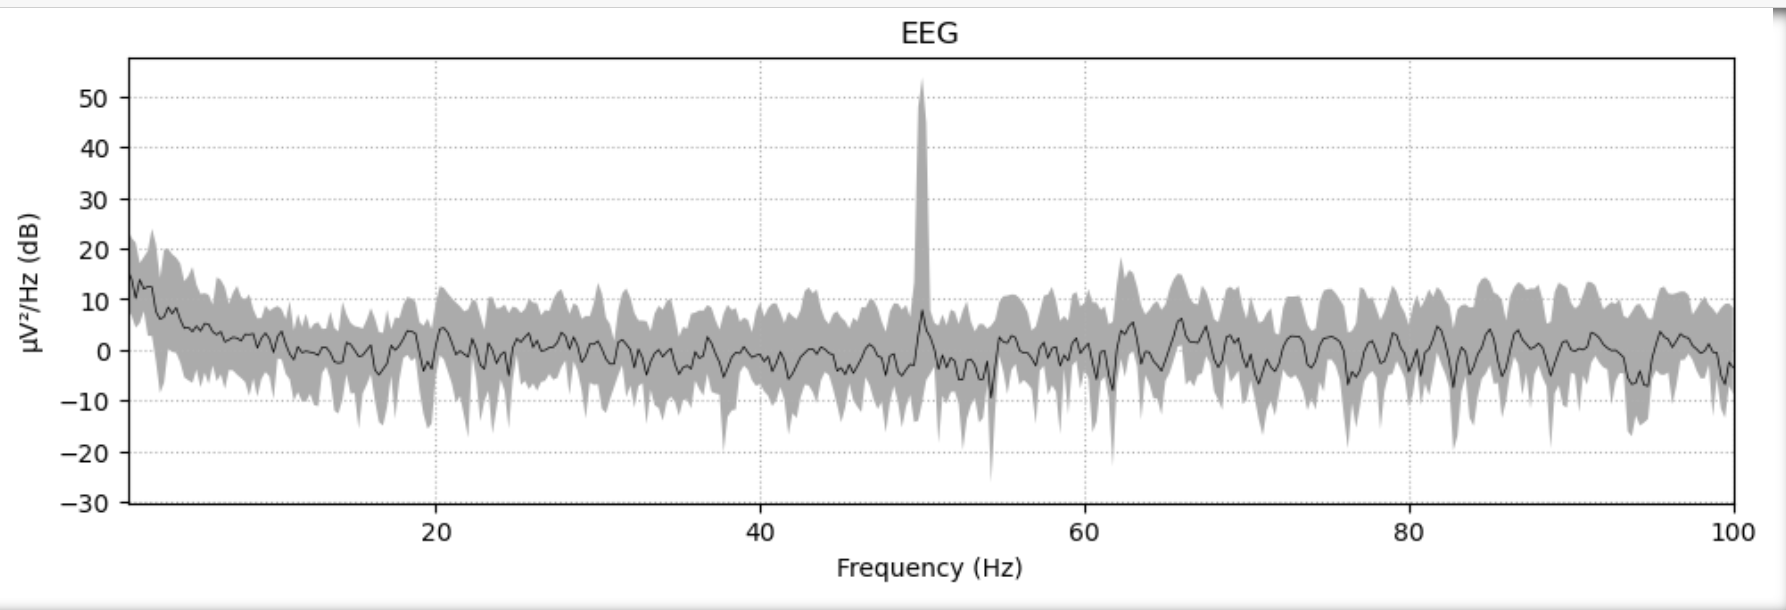
\includegraphics[width=\textwidth]{figures/background_psd_plot.png}  
    \caption{EEG signal strength against frequency, 0–100 Hz, showing 50 Hz line noise.}
    \label{fig: PSD of line noise}
\end{figure*}

As previously stated, EEG data is susceptible to interference from electrical appliances, leading to noise mostly at frequencies of 50 Hz in Europe (as depicted in Figure \ref{fig: PSD of line noise}) and 60 Hz in the USA. This phenomenon arises due to the prevailing power line frequencies in the corresponding geographical areas. Therefore, employing a notch filter, specifically a band-stop filter with a small stopband centered at 50 Hz or 60 Hz, is common practice to eliminate line noise effectively \cite{delorme2023eeg}. Other filtering methods include low pass filtering, which entails the elimination of higher frequencies, high pass filtering, which eliminates frequencies below a specific threshold while preserving high frequencies \cite{gonccales2021effects}; and bandpass filtering, which combines the above filtering techniques. 
The bandpass filter selectively keeps frequencies within the specified upper and lower bounds while eliminating frequencies that do not fall within this range. Furthermore, the Butterworth filter, known for its maximally flat magnitude in the passband, is widely used in pre-processing EEG data \cite{survey_brain_biometrics}.       
\subsection{Artifacts Rejection}
One often employed approach for mitigating physiological artifacts is discarding EEG data over a predefined threshold of EEG voltage \cite{jung2000removal}, such as 100$\mu$V since physiological artifacts generally exhibit significantly greater magnitudes in comparison to cerebral activity \cite{survey_brain_biometrics}. However, a more sophisticated method of rejecting artifacts is the peak-to-peak rejection method. This approach involves identifying and removing EEG segments that surpass a predetermined voltage range. This range is commonly determined by measuring the peak-to-peak amplitude, which is the difference between the highest positive and lowest negative deflections within a specific time frame \cite{luck2014introduction}. While the peak-to-peak rejection technique efficiently eliminates noisy signals, its application can inadvertently remove substantial valuable EEG data. This outcome is particularly possible when the method is not executed after meticulous assessment, as the amplitude of EEG signals can significantly differ based on experimental configurations and the characteristics of the utilized headsets.  

\subsection{Independent Component Analysis}
The Independent Component Analysis (ICA) is an innovative signal processing technique that enables the separation of sources that have been linearly mixed at the sensors. This separation is achieved by assuming simply the statistical independence of the sources \cite{vigario2000independent}. Accroding to Hyv\"arinen \textit{et al.} \cite{hyvarinen1999fixed}, the ICA algorithm can be defined by the following equation.
\begin{equation}
S \cdot X=U
\end{equation}
where S is the unmixing matrix, X is the signal of EEG channels where each row corresponds to a sensor channel , and each column corresponds to a time point in the recorded signals and U represents the matrix of the estimated independent source signals. This method enables the segregation of EEG signals from noise and randomly mixed signals, contributing significantly to enhanced signal quality and analysis .  

%One often employed approach for mitigating physiological artifacts is discarding EEG data over a predefined threshold of EEG voltage \cite{jung2000removal}, such as 100$\mu$V since physiological artifacts generally exhibit significantly greater magnitudes in comparison to cerebral activity \cite{survey_brain_biometrics}. However, a more sophisticated method of rejecting artifacts is by employing peak to peak rejection. This approach involves identifying and removing EEG segments that surpass a predetermined voltage range. This range is commonly determined by measuring the peak-to-peak amplitude, which is the difference between the highest positive and lowest negative deflections within a specific time frame \cite{luck2014introduction}. 

% \item Physiological artifacts are particularly tricky as they emanate from the body's inherent processes. For instance, the electric fields produced during eye movements or blinks, heartbeats, muscle contractions, or even perspiration can introduce significant noise into the EEG signals. These artifacts often cause substantial voltage fluctuations that can easily exceed an amplitude of 100$\mu$V, thus, effectively masking the true EEG signal.

% \item Line noise is a prevalent artifact in EEG signals, generated by electronic equipment present during the EEG experiment. The circulating electrical current in the building's electrical system gives rise to an electromagnetic interference known as "line noise". This interference, detected by the EEG cables, has a frequency determined by the local power grid, usually 50 Hz in Europe and 60 Hz in the USA.
% \end{itemize}
\section{EEG Features}
\label{sec:Background:EEG Features}
safdds
\subsection{Auto regressive Coefficients}
%The AR model is a type of random process where the output variable is linearly dependent on its prior values as well as a stochastic term that is not completely predictable \cite{survey_brain_biometrics}, and the following equation defines it:
The Autoregressive (AR) model is a stochastic process in which the output variable is linearly influenced by its previous values, together with an unpredictable stochastic term \cite{survey_brain_biometrics}. The following equation can mathematically represent the AR model: 
%The Autoregressive (AR) model is a type of stochastic process wherein the output variable is impacted linearly by its past values and an unpredictable stochastic component \cite{survey_brain_biometrics}. The subsequent equation can be employed to express the AR model formally: 
\begin{equation}
x(n)=-\sum_{i=1}^p a_i x(n-i)+e(n) .
\end{equation} 
%where x(n) is the current value of one channel, ${a_{i}$ is the AR coefficients at delay i, e(n) is the error at time n, and p is the order.
where x(n) represents the current value of a particular channel, ${a_{i}$ denotes the AR coefficients at specific delay i, e(n) represents the error at time n, and p represents the order of the model.

Yule walker and Burg's method
    
\subsection{Power Spectral Density}
The Power Spectral Density (PSD) is employed to represent the power distribution of a signal across different frequency points \cite{zhang2021review}.

Fourier Transformation, Discrete Fourier Transformation and welch's periodgram.  
\subsection{Common Spatial Patterns}
\subsection{Time-Frequency Analysis}
\subsection{Wavelet Transform}
\subsection{Statistical Features}

\section{Authentication Algorithms}
\label{sec:Background:Authentication Algorithms}
\begin{itemize}
    \item Linear Discriminant Analysis
    \item Logistic Regression
    \item Support Vector Machine
    \item K Nearest Neighbour
    \item Gaussian Naive Bayes
    \item Deep Learning
\end{itemize}
% \subsection{Common Performance Metrics}
% \begin{itemize}
%     \item Confusion metrics
%     \item Accuracy, Precision, Recall, F1-Score
%     \item EER
%     \item ROC-Curve
%     \item DET-Curve
%     \item FAR and FRR
% %\end{itemize}
